\section{IoTDSL}
\label{sec:IoTDSL}

\begin{figure}%
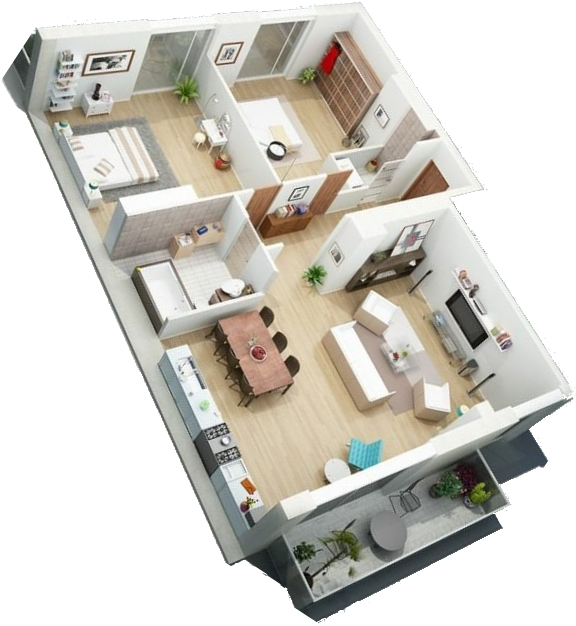
\includegraphics[width=\linewidth]{MaisonSansDevices.png}%
\caption{Alice's smart home equipped with various devices.}%
\label{fig:RE}%
\end{figure}

Building a well-calibrated \DSL is known to be difficult and error-prone. It usually requires a large expertise on a domain and its many variations before a consensus on which concepts are important and how to effectively represent them emerge. Fortunately, \MDE technologies operated substantial breakthrough over the past decade, allowing language designers to easily define their own \DSL structures and user interfaces. A \DSL is often required to exhibit a visual syntax, allegedly to simplify its understanding and manipulation by end-users. However, in order to obtain faster a functional prototype, we chose to start from a textual syntax, which is easier to manipulate and evolve for language designers. Ultimately, we plan to propose a visual syntax: the transition should be facilitated since our \DSL is developed from the start in GeMoC \cite{combemale-14}, an \textsc{Mde} framework that supports both visual and textual representations as concrete syntaxes and maintains a full synchronisation between both versions.

Based on the concerns and challenges identified in section~\ref{sec:Context-Challenges}, we now introduce \IOTDSL, our \DSL devoted to facilitate the high-level manipulation of \IOT systems. At the heart of \IOTDSL are two governing principles. First, we promote a clean separation of concerns for all aspects the \DSL has to handle. As a consequence, our \DSL's structure embeds several sublanguages that are composed together to form \IOTDSL. We believe this approach to be scalable, and to support a well-controlled independent evolution of each concern without impacting the other aspects, since those aspects are composed through well-defined interfaces. Second, our \DSL relies on events, a natural paradigm for specifying various models of interactions that is classically used in embedded and critical systems, and where a clear separation between the system and its environment is performed, helping us enforce separation of concerns.

Despite its early stages of development, \IOTDSL showed its ability to appropriately capture the definition of small-scale \IOT systems. We first extract a simple scenario from our project at the University of Namur to demonstrate typical usages of \IOT systems deployed inside a house. We then simultaneously explain each part of the definition of \IOTDSL, and illustrate it in dedicated examples.

\subsection{Running Example}
\label{sec:IoTDSL-Example}

To illustrate our proposal, we consider a smart home equipped with several devices, just like Alice's situation in Section \ref{sec:Context-Challenges}, as illustrated in Figure \ref{fig:RE}. At the entrance, the door is equipped with a lock detector, allowing to know when the door is opened or closed. The hallway contains motion detectors, so that the lights in the hallway as well as in the living room automatically switch on when she enters her house. Furthermore, the living room also contains a presence detector because Alice wants the temperature to be automatically monitored when she's occupying the room, being maintained between 20°C and 22°C; otherwise, when she is not home, the temperature may not drop below 16°C. For security reasons, Alice's kitchen contains a smoke detector and a temperature monitor. When she cooks, it happens that she burns something; but she wants to make sure to detect any departing fire: she considers a critical situation when the temperature remains above 40°C consistently during five minutes while there is also smoke in the kitchen. 

% for placement reasons
\begin{figure*}%
  \centering  
  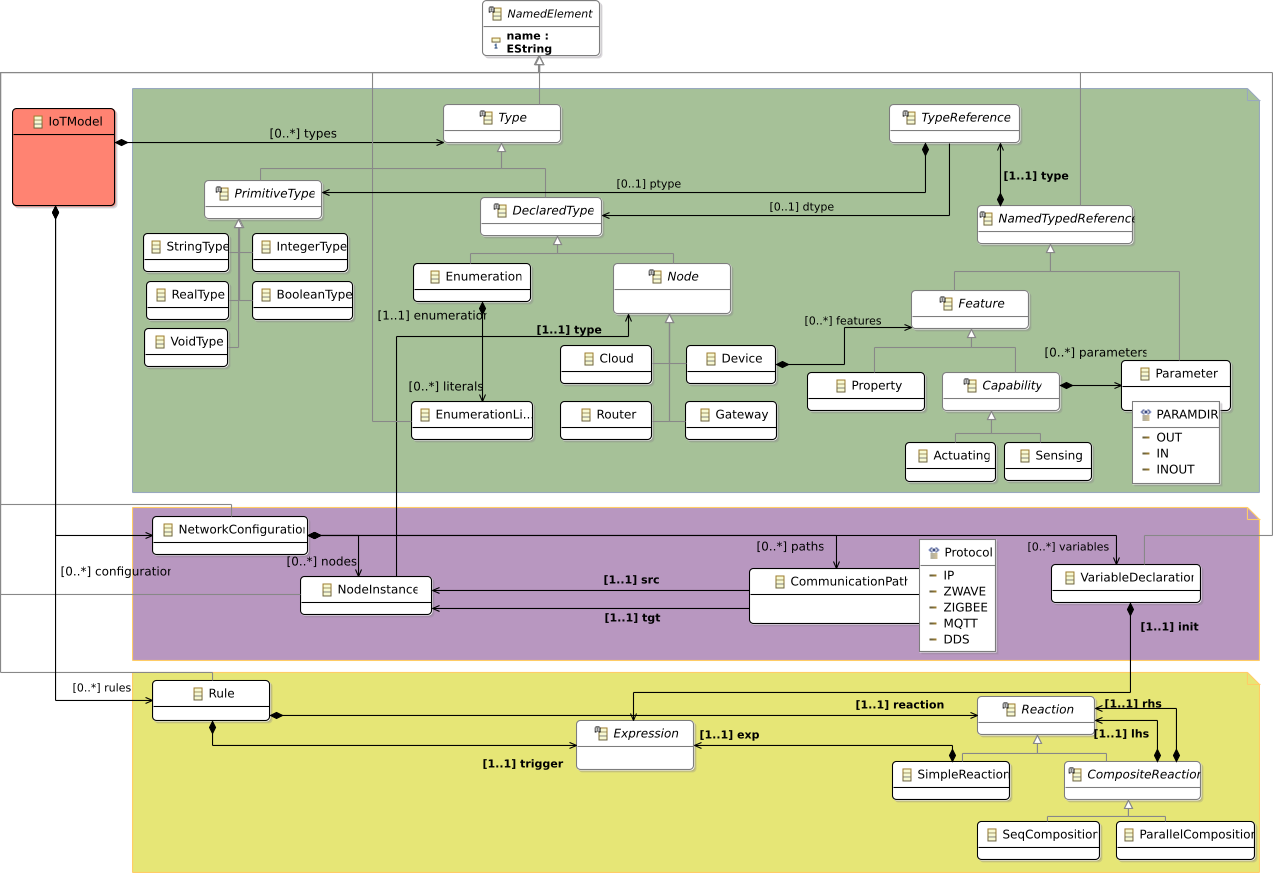
\includegraphics[width=.75\linewidth]{IoTDevice-MM.png}%
  \caption{Metamodel of \IOTDSL, separated in three concerns: \emph{Type Definition} captures devices' capabilities (top green part), \emph{Network Configuration} details how device instances are connected to each others (middle purple part), \emph{Business Rules} defines the functionalities expected from the IoT installation (bottom yellow part).}%
  \label{fig:IoTDevice-MM}%
\end{figure*}

Figure \ref{fig:RE} shows how the various devices are physically distributed inside an archetypal representation of a smart home, and how each device communicates with a centralised gateway. In our \DSL, the gateway concentrates the data received from the devices deployed inside the home, and keeps the business logic running, \textit{i.e.} receiving data from and acting through the devices. 

\subsection{Type Definition}
\label{sec:IoTDSL-Type}
 
In this section, we define \IOT devices' types, \textit{i.e.} which capabilities are available to the users in terms of environment sensing and actuating. In our scenario, type definitions either come from an advanced user who is able to reason properly about a particular device and extract the relevant information, or from a preexisting devices database, either being an actual repository the system is connected to, or a library of \textit{devices-off-the-shelf}. The concepts dedicated to type definition are shown in Figure~\ref{fig:IoTDevice-MM} (green background). This part is similar to the notion of \textsf{Classifier} in \textsc{Mof}-like languages: a \textsf{Type} is either a \textsf{PrimitiveType} (integers and real numbers, strings and booleans), or a user-defined \textsf{DeclaredType}. We distinguish between general \textsf{Gateway}s, which centralise information and processing, from \textsf{Node}s, which possess capabilities and are deployed in the environment. A \textsf{Capability} is basically a \textsc{Mof}-like operation with a signature, expressed through a list of \textsf{Parameter}s that either capture data from the environment, or act on it. A \textsf{Node} can mix both kinds of capabilities, allowing us to represent in a uniform fashion composite devices that expose complex behaviours.

For now, type definitions are defined as specific files that can be imported and combined easily within an \IOT specification. We plan to propose a graphical interface to facilitate the browsing and integration of library components into \IOT systems.

Listing~\ref{lis:RE-TypeDeclarations} shows how the devices used in the Running Example are declared in \IOTDSL. Each device is introduced by the keyword \textsf{device}, has a name and capabilities that correspond to reporting events (\textsf{sensing}) or operating over the environment (\textsf{actuating}). A special device, introduced by the keyword \textsf{gateway}, centralises data from all devices connected to it (cf. Section \ref{sec:IoTDSL-NetworkConfiguration}). Note that this is the visible part of \IOTDSL: in the background, the events declared for all devices need to be mapped to concrete low-level events that the devices actually use. For that purpose, \IOTDSL contains a mapping language aimed at reconciling high- and low-level events that is not detailed here for space reasons.

\begin{center}
\begin{minipage}[t]{.42\linewidth}
\begin{lstlisting}[language=iotdsl]	
device DoorLock {
  sensing opened()
  sensing closed()
}
device PresenceDetector {
  sensing detected()
  actuating isPresent()
}
device LightBulb {
  actuating on()
  actuating off()
  actuating blink()
}	
device TempSensor {
  sensing getTemp()
}
\end{lstlisting}
\end{minipage}\hfill
\begin{minipage}[t]{.49\linewidth}
\begin{lstlisting}[language=iotdsl, firstnumber=17]
device Heater {
  actuating warm(delay:Integer)
  actuating stop()
}
device Alarm {
  actuating sound()
  actuating call(msg:String)
}
device Timer {
  actuating reset()
  actuating set(delay:Integer)
  sensing timeout()
}
gateway Central


\end{lstlisting}
\end{minipage}
\captionof{lstlisting}{Type declarations in \IOTDSL: \textsf{sensing} or \textsf{actuating} capabilities as high-level events.}
\label{lis:RE-TypeDeclarations}
\end{center}


\subsection{Network Configuration}
\label{sec:IoTDSL-NetworkConfiguration}

The configuration-related constructs are specified in the purple-part of Figure~\ref{fig:IoTDevice-MM}. A concrete device is materialised by a \textsf{NodeInstance} and is typed by an abstract \textsf{Node}, \textit{e.g.} a \textsf{Device} or a \textsf{Gateway}. Instances may communicate with other \IOT devices through predefined \textsf{CommunicationPath}s. Such paths define, among others, one or more protocols used for communication. We actually rely on existing platforms, such as OpenRemote~\cite{fixme} or SmartThings~\cite{fixme} to handle the intricate details of the communication protocols since these details are, from an end-user viewpoint, technical aspects rather than essential matters. By knowing which protocols are used between each pair of devices, we can perform data conversion in the proper format required by the protocols automatically: most of those protocols are already implemented in General-Purpose Programming Languages (\textsc{Gpl}s), like Java or C, to name a few of them.

\begin{lstlisting}[label=lis:RE-Network,language=iotdsl,caption=Network Configuration for Alice's House]	
configuration MyHome {
  node gw 					   : Central
  node livingTemp      : TemperaturSensor
  node kitchenTemp     : TemperaturSensor
  node livingHeater    : Heater
  node frontdoor       : DoorLock
  node corridorLight   : LightBulb
  node livingLight     : LightBulb
  node timer           : Timer
  node alarm           : Alarm
  node corridorDetector: PresenceDetector
  node livingDetector  : PresenceDetector

  from livingTemperature to gw via MQTT
  from HomeTemperature to gw via DDS
  from livingHeater to gw via DDS
  from frontdoor to gw via MQTT
  from light to gw via MQTT
  from timer to gw via DDS
  from alarm to gw via DDS
  from bodydetector to gw via MQTT
}
\end{lstlisting}	

From a practical point of view, we can easily imagine that network configurations are automatically established if devices follow the recommendation of discovery protocols~\cite{}. By concentrating the connections on a gateway in charge of centralising the joining and leaving devices, \textit{e.g.}, phones that enter or leave a house, it becomes possible to gather information on new devices and connect them appropriately to other devices in the network according to their capabilities, communication protocols, and so on. Although \IOTDSL empowers \textsf{Node}s to be passed as \textsf{Parameter}s, enabling devices' definition to be discovered thanks to the \textsf{Gateway}.

Listing~\ref{lis:RE-Network} shows the connection between the devices presented in Figure~\ref{fig:RE}. A specific device is considered as an instance of a defined type such that particular devices with the same set of capabilities may be distinguished via identifiable references. Communications are purely declarative and only mention the protocol type (introduced by the \textsf{via} keyword). Note that we added an extra instance \textsf{timer : Timer} used to simulate time elapsing. This \textit{pseudo} device is used to artificially set a clock time, whose behaviour is directly linked to the supporting platform of the gateway's for time management.
	
\subsection{Business Rules}
\label{sec:IoTDSL-BusinessRules}

This last part of our \DSL is the heart of \IOT systems manipulation and is detailed in the in the bottom yellow part of Figure~\ref{fig:IoTDevice-MM}. It relies on an event-based framework consisting of a set of \textsf{Rule}s that implement various functionalities an end-user wants to achieve. Rules' \textsf{trigger}s are cyclically evaluated against the surrounding environment. Whenever a \textsf{trigger} \textsf{Expression} becomes true, it executes the appropriate \textsf{reaction} associated to the rule. A \textsf{trigger} is defined as an expression, whose precise definition is omitted here since it simply follows any expression language available in \textsc{Gpl}s for navigating nodes and evaluating boolean or arithmetic expressions\footnote{Note that the evaluation of the \emph{absence} of events is left for future work, since this is a rather tricky problem. As a consequence, the current expression language does not integrate boolean negation yet.}.A \textsf{reaction} defines a sequential or parallel combination of capabilities, enabling to sort actions by, or require data from some identifiable devices. An typical \textsf{reaction} may be to switch on all lights in a house, or only the ones of a certain type.

For now, our approach is purely middleware-oriented: rules are gathered into a gateway. For efficiency and resource consumption reasons, we are also exploring how to automatically identify parts of the business logics that can be exported to advanced nodes with sufficient processing and power resources, in order to lower network and gateway overuses.

We now explain how the scenario presented in the running example is translated in business rules in \IOTDSL. We identified three different situations where Alice needs to specify what she expects from the devices of her house:
\begin{enumerate}
	\item When Alice enters home (and thus opens the front door), she wants the lights in the hallway and the living room to be automatically switched on. 

\begin{lstlisting}[language=iotdsl]
rule SwitchLightsWhenEnter:
  when (frontdoor.opened() and 
      after corridorDetector.detected()) do {
    corridorLight.on() || livingLight.on()
  }
\end{lstlisting}	
	
	\item When Alice is in the living room, the temperature inside the room should be maintained between comfortable temperatures; whereas when she is not, the temperature should not drop below 16°C.
	
	
\begin{lstlisting}[language=iotdsl]
rule PresentInLiving:	
  when (presenceTimer.timeout()) do {
     livingDetector.isPresent() || 
       (presenceTimer.reset ; presenceTimer.set(TIMEDETECT))
  }
rule MonitorLivingTempInStop:
  when (livingDetector.detected() 
      and livingTemp.getTemp > IN_MAX) do {
    livingHeater.stop()
  }
rule MonitorLivingTempInStart:
  when (livingDetector.detected() 
      and livingTemp.getTemp < IN_MIN) do {
    livingHeater.warm(TIMEHEAT)
  }
rule MonitorLivingTempOutStart:
  when (presenceTimer.timeout() 
      and before livingTemp.getTemp < OUT_MIN) do {
    livingHeater.warm(TIMEHEAT)
  }
\end{lstlisting}
	
	\item There is a critical fire situation when smoke is detected in the kitchen while temperature is upper 40°C for at least five minutes.
\end{enumerate}


These rules show some particularities of \IOTDSL's Rule language. First, it is possible to define local or global variables and reuse them as part of parameters or expressions (cf. Rules \textsf{PresentInLiving} or \textsf{MonitorLivingInStop}, among others). Second, it is possible to compose reactions either in sequence (class \textsf{SeqComposition} in the metamodel of Figure \ref{fig:IoTDevice-MM}, textually represented as \textsf{\textbf{;}}) or in parallel (class \textsf{ParallelComposition}, represented as \textsf{\textbf{||}}), like Rule \textsf{PresentInLiving} demonstrates. Third, \IOTDSL's expression language integrates a simple mechanism for events time management: the \textsf{before} and \textsf{after} event modifiers check that an event happens in a reasonable time windows before/after the one it is combined to (in Rules \textsf{SwitchLightWhenEnter} and \textsf{MonitorLivingTempOutStart}, events are combined with \textsf{and} for checking quasi-simultaneity). Fourth, because \IOTDSL cannot check the non-occurrence of events, time management is crucial for ensuring a sound detection of interesting non-events: for example here, Rule \textsf{PresentInLiving} is used to periodically check for presence in the living room (with the actuation \textsf{isPresent()}); but when nobody is detected, we still have to maintain the temperature above \textsf{OUT\_MIN} = 16°C. By detecting that \textsf{timeout()} occurred previously, we still are capable of adjusting the living room temperature adequately.
